
\chapter{Implementación de la Radio Definida por Software en sistemas de radiodifusión}

Este capítulo tiene el fin de estudiar lo que significa Software Defined Radio (SDR) y un tipo de hardware usado en SDR. Con el fin de lograr que el estudiante tenga contacto con un hardware real, hemos seleccionado el USRP-2920 de la empresa National Instruments, pero también se busca generalizar el conocimiento sobre ese hardware en forma de modelos más generales que le brinde al estudiante la capacidad de descubrir y comprender cualquiera de los tipos de hardware existentes. El mayor ènfasis se hace en que estudiante conozca lo que un hardware SDR representa. 

%%%%%%%%%%%%%%%%%%%%%%%%%%%%%%%%%%%%%%%%%%%%%%%

\section{Radio Definida por Software en Modo de Red}

El término Modo de Red o “modo Network” es muy usado en los productos de la empresa Ettus, la cual a su vez pertenece a National Instruments, pero este modo corresponde la configuración más común en los laboratorios experimentales por ser la solución más económica y a la vez más potente. Consiste en lograr un complemento perfecto entre un hardware SDR y un computador con el software apropiado. El término network es usado debido a que el hardware se conecta al computador usualmente por un puerto Giga Ethernet de manera directa. En principio, no se descarta que esa conexión sea por Wi-Fi o que los componentes estén ubicados en lugares remotos distantes entre sí, unidos por Internet, pero esto no es usual pues entre el hardware y el computador se requiere enviar información muy pesada en tiempo real. \\


%\setcounter{figure}{57}
\begin{figure}[h!]
	\captionsetup{justification = raggedright, singlelinecheck = false}
	\caption{Un sistema de comunicaciones punto a punto Full Duplex.} 
	\centering
	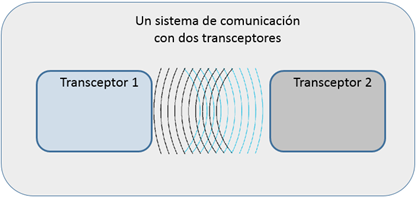
\includegraphics[scale=0.8]{Imagenes/Full-duplex.png}
	\label{fig:Full-duplex}
%		\captionsetup{justification=raggedright,font={scriptsize,bf,it}}
%		\caption*{fuente: http://superkuh.com/rtlsdr.html}
\end{figure}

\vspace{200px}
\begin{figure}[h!]
	\captionsetup{justification = raggedright, singlelinecheck = false}
	\caption{Un transceptor (en inglés Transceiver).} 
	\centering
	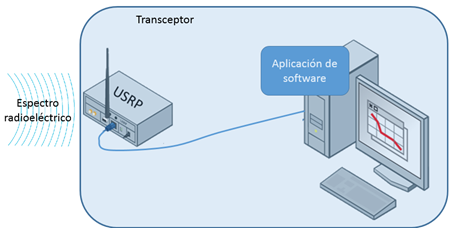
\includegraphics[scale=0.8]{Imagenes/Transceptor.png}
	\label{fig:Transceptor}
	%		\captionsetup{justification=raggedright,font={scriptsize,bf,it}}
	%		\caption*{fuente: http://superkuh.com/rtlsdr.html}
\end{figure}

USRP (Universal Software Radio Peripheral) es el término usado por la empresa Ettus para denominar el hardware de una solución SDR. Como se muestra en la figura anterior, en el USRP se concentra la componente hardware del sistema de comunicación y en el computador la componente del software. Lo que viaja por el cable que une estos componentes es precisamente la Envolvente Compleja, no sin antes ser adaptada al protocolo Ethernet.\\

Para los USRP que solo funcionan en modo Network, se usa una nomenclatura especial, se considera que pertenece a la serie Nx, donde la N significa Network y la x unos números seriales. Algunos ejemplos son:  USRP N200, USRP N210. Sin embargo, como la empresa Ettus fue adquirida por National Instruments (NI), esta empresa está usando otra nomenclatura como: NI USRP 2920, NI USRP 2921, NI USRP 2922, NI USRP 2930, NI USRP 2932. Ese cambio de nomenclatura es aplicado por NI para indicar que estos equipos funcionan con LabView que es la plataforma de NI que ahora incursiona en SDR. Una comunicación completa en Modo Network se presenta en la figura \ref{fig:Modelo-capas}.\\

\begin{figure}[h!]
	\captionsetup{justification = raggedright, singlelinecheck = false}
	\caption{Modelo de capas de un sistema de comunicación con USRP en Modo Network.} 
	\centering
	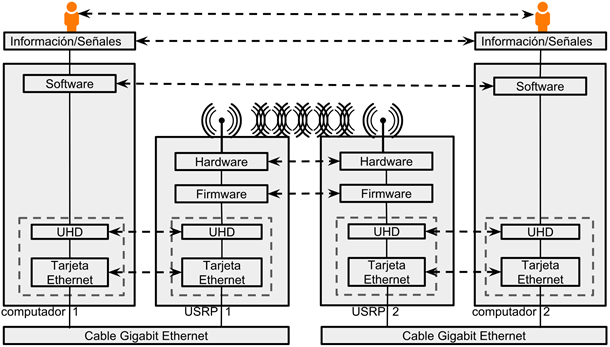
\includegraphics[scale=0.8]{Imagenes/Modelo-capas.png}
	\label{fig:Modelo-capas}
	%		\captionsetup{justification=raggedright,font={scriptsize,bf,it}}
	%		\caption*{fuente: http://superkuh.com/rtlsdr.html}
\end{figure}

%%%%%%%%%%%%%%%%%%%%%%%%%%%%%%%%%%%%%%%%%%%%%%%%%%%

\section{Un equipo SDR parara Modo de Red. El NI USRP-2920}

El NI USRP-2920 es un ejemplo típico de un hardware pensado en una solución de comunicación basada en SDR en modo network. vale la pena usarlo como ejemplo para conocer lo que este tipo de equipos usualmente contiene. \\

\begin{figure}[h!]
	\captionsetup{justification = raggedright, singlelinecheck = false}
	\caption{Foto del NI USRP-2920.} 
	\centering
	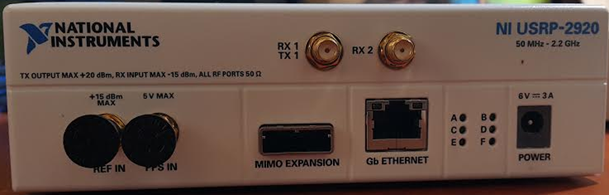
\includegraphics[scale=0.8]{Imagenes/USRP-2920.png}
	\label{fig:USRP-2920}
	%		\captionsetup{justification=raggedright,font={scriptsize,bf,it}}
	%		\caption*{fuente: http://superkuh.com/rtlsdr.html}
\end{figure}

Es importante, tener claro desde un comienzo que estos USRP son construidos por la empresa \underline{Ettus Research}. Pero esta empresa fue adquirida en el 2015 por la empresa National Instruments (NI). De esta manera se entiende por qué un mismo hardware tiene dos nombres diferentes: uno que le da Ettus y otro que le da NI. \textbf{Es asì como el NI USRP 2920 de National Instruments corresponde al USRP N210 de Ettus}, donde la N indica que se trata de un equipo que funciona en modo Network. El equipo viene un software de NI que permite configurar el equipo con el driver que le permite actuar como NI USRP 2920 o bien con el driver que le permite actuar como USRP N210. El primer caso se usa cuando el equipo se usa con LabView sobre Windows, mientras el segundo, con GNU radio sobre Ubuntu. \\

El	\textcolor{red}{\href{http://www.ni.com/pdf/manuals/375839a.pdf}{manual de este equipo, en este enlace}}, es suficiente para comprender lo que el equipo representa externamente, así como sus especificaciones técnicas y cuidados de uso. Nos detendremos más bien en el esquema interno.\\

\vspace{400px}
\begin{figure}[h!]
	\captionsetup{justification = raggedright, singlelinecheck = false}
	\caption{Modelo de capas del NI USRP 29xx visto por capas. En color naranja: bloques de software embebido. En color verde: Hardware con parámetros controlables por computador. Blanco: Hardware no controlable.} 
	\centering
	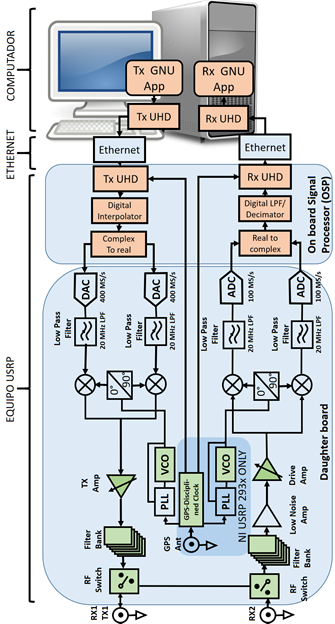
\includegraphics[scale=0.8]{Imagenes/Modelo-29xx.png}
	\label{fig:Modelo-29xx}
		\captionsetup{justification=raggedright,font={scriptsize,bf,it}}
			\caption*{fuente: FALTA \textbf{Nota:} Según el manual del NI-USRP 2920 no es claro que tenga un banco de filtros}
\end{figure}

En los siguientes capítulos, el término “Usuario P” se refiere a la persona que está sentada en el computador, desarrollando una aplicación en GNU radio o usando una para contactar el USRP. \\

\subsection{El receptor del NI USRP-2920}

Como puede apreciarse, la parte receptora consiste en una o dos antenas que son conectadas por el RF switch. En muchos USRP la señal pasa inmediatamente por un banco de filtros que resultan sintonizados mediante las órdenes que da el Usuario P desde la aplicación ubicada en el computador. La señal es luego amplificada en el Low Noise Amp. La señal sigue a un amplificador que puede ser configurado por el usuario P desde la aplicación. El esquema que sigue es lo que en el primer capítulo hemos llamado Down Converter, en el cual la frecuencia del Oscilador controlado por voltaje (VCO) puede ser configurada desde la aplicación, pero no los parámetros del Low Pass Filter, que tiene un ancho de banda fijo, inmodificable, de 20 MHz. \\
El Usuario P tampoco puede modificar los parámetros del Conversor Análogo Digital (ADC), que muestrea la señal a su entrada a una rata fija, invariable de 100 MS/s y además la cuantiza a 14 bits/muestra. El Usuario P debe jugar con la ganancia o la atenuación para poder aprovechar todos los 14 bits por muestra, pues la señal entrante es muy débil y no alcanzaría a levantarse de manera suficiente. Pero también es necesario tener en cuenta que una sobre amplificación puede crear también un problema, el de saturación, como se muestra en las siguientes dos figuras.

\begin{figure}[h!]
	\captionsetup{justification = raggedright, singlelinecheck = false}
	\caption{Señal a la entrada del cuantizador.} 
	\centering
	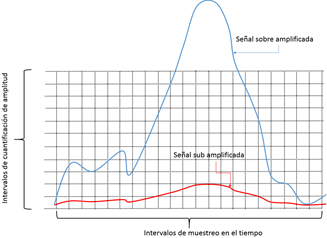
\includegraphics[scale=1]{Imagenes/Senal-entrada.png}
	\label{fig:Senal-entrada}
	%		\captionsetup{justification=raggedright,font={scriptsize,bf,it}}
	%		\caption*{fuente: http://superkuh.com/rtlsdr.html}
\end{figure}


\begin{figure}[h!]
	\captionsetup{justification = raggedright, singlelinecheck = false}
	\caption{Señal a la salida del cuantizador.} 
	\centering
	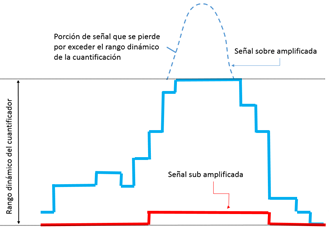
\includegraphics[scale=1]{Imagenes/Senal-salida.png}
	\label{fig:Senal-salida}
	%		\captionsetup{justification=raggedright,font={scriptsize,bf,it}}
	%		\caption*{fuente: http://superkuh.com/rtlsdr.html}
\end{figure}

Por esta razón, es ideal que la señal resultante después de la amplificación quede con magnitud 1 o incluso 0,8, ya que el rango dinámico del ADC es 1 Vp-p, para el caso del NI USRP 2920. Así, las amplitudes de la componente I y la Q se puede deducir de la magnitud $\sqrt{I_{max}^{2} + Q_{max}^{2}} = 1$.\\

\subsubsection{Cálculo de la frecuencia de muestreo para un NI USRP.}

La señal pasa luego a la FPGA (la tarjeta madre), donde está el OSP (Onboard signal processor) que tiene algunos elementos de procesamiento digital, filtra la frecuencia central, de modo que no aparezca allí un delta que corresponde a la portadora. Pero también en el OSP se le aplica a la señal una decimación, combinado con un filtrado digital, para bajar la rata de muestreo de la señal I/Q para que cumpla con los deseos del programador que especificará un ancho de banda deseado que, en términos de frecuencia de muestreo, resultará en un valor que para el NI USRP 292x está entre 200 kS/s y 25 MS/s. Debido a las limitaciones del computador y la calidad del cable usado para unir el USRP con el computador, el Usuario P puede considerar que el ancho de banda pasobandas está entre 200 kHz y 20 ó 25 MHz, como se muestra en la siguiente figura. \\


\begin{figure}[h!]
	\captionsetup{justification = raggedright, singlelinecheck = false}
	\caption{Ancho de banda real que puede alcanzar el NI USRP 2920 con respecto a las capacidades de la tarjeta hija} 
	\centering
	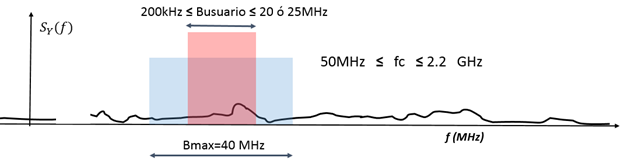
\includegraphics[scale=1]{Imagenes/Ancho-banda-real.png}
	\label{fig:Ancho-banda-real}
	%		\captionsetup{justification=raggedright,font={scriptsize,bf,it}}
	%		\caption*{fuente: http://superkuh.com/rtlsdr.html}
\end{figure}

Ese ancho de banda se puede configurar en los bloques digitales alojados en el OSP. Esto ocurre de manera indirecta, cuando el Usuario P selecciona un el Coeficiente de Decimación $K_{d}$ para el bloque Digital LPF/decimator con el fin de bajar la frecuencia de muestreo. Es importante tener en cuenta que, usualmente ese coeficiente es un número entero y a la vez potencia de 2, de modo que: \\

\begin{equation} \label{captres_uno}
 K_{d} =2^{m}, donde m es entero positivo. \end{equation}

Los experimentos desarrollados por el autor, con el NI USRP 2920, muestran que, aunque el sistema acepta cualquier valor entero que sea par y positivo para ese coeficiente, si no se escoge como se señaló, se deforma el espectro de la señal que sale del decimador respecto a la que recibe el decimador. \textbf{El autor también demostró que con el NI USRP 2920, hay un tope máximo para ese coeficiente y es 512.} Eso significa que así como el equipo tiene un tope máximo para la frecuencia de muestreo de 100 MSps, también tiene un tope mínimo de 195,3125 kS/s, ósea $100e^{6}/512$. Esto también significa que, el mínimo ancho de banda que el USRP captura en pasobandas es 195,3125 kHz, que equivale a 97,65625 kHz en bandabase. \\

La señal resultante es luego enviada por el cable gigabit ethernet. En conclusión, el USRP captura una señal en toda la banda de 40 MHz, pero la procesa para enviar a la Rx GNU App el ancho de banda que el Usuario P configure en función del Coeficiente de Decimación. También es claro que el usuario está obligado a realizar la decimación, ya que de otra suerte, estaría obligando al USRP a entregar una rata de muestras que no es soportada por el sistema que une el USRP con el computador, o incluso por la capacidad del mismo computador. \\

\vspace{250px}
\begin{figure}[h!]
	\captionsetup{justification = raggedright, singlelinecheck = false}
	\caption{Análisis en banda base de frecuencias de muestreo y anchos de banda que se manejan en el USRP 2920 en el modo de recepción.} 
	\centering
	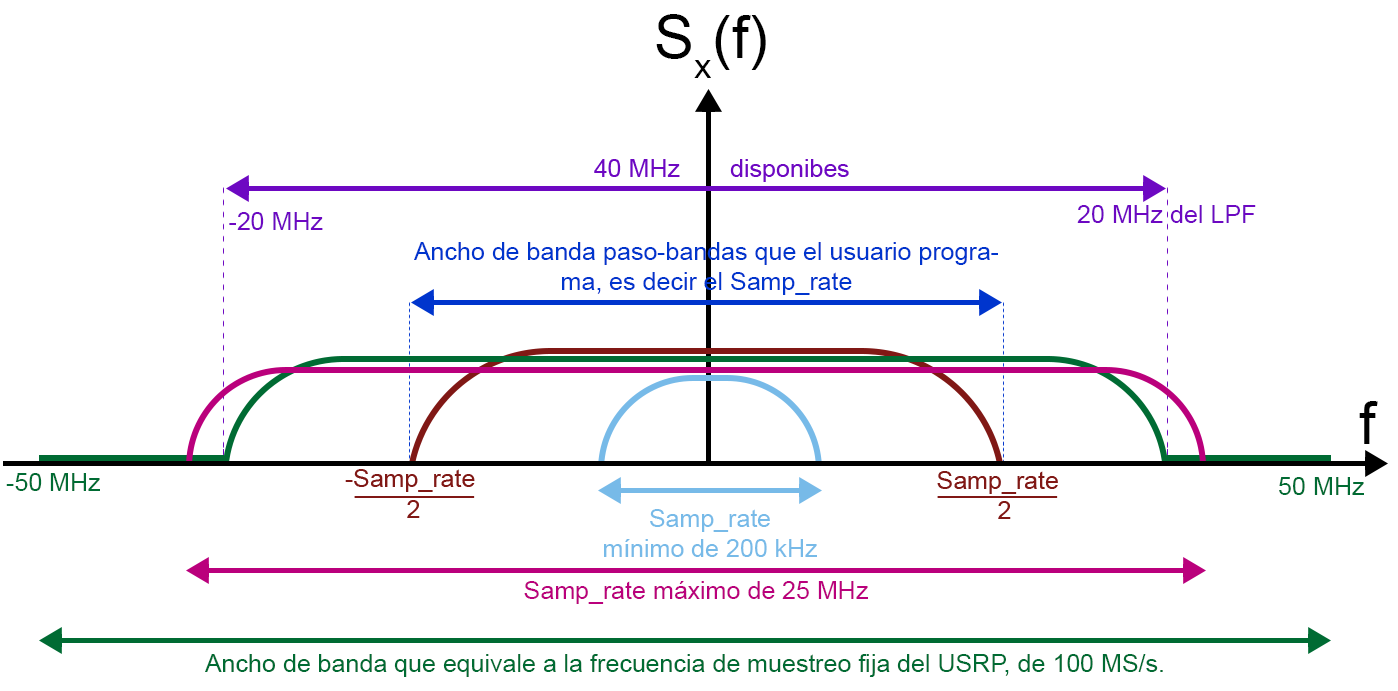
\includegraphics[scale=0.3]{Imagenes/Analisis-banda.png}
	\label{fig:Analisis-banda}
	%		\captionsetup{justification=raggedright,font={scriptsize,bf,it}}
	%		\caption*{fuente: http://superkuh.com/rtlsdr.html}
\end{figure}

En la figura anterior, vemos que la frecuencia de muestreo de 100 MS/s que por defecto maneja el DAC está sobredimensionada con respecto al ancho de banda del filtro analógico paso bandas usado como parte del down converter que es de 20 MHz, para capturar una señal de hasta 40 MHz. Pero al programador le interesa. Pero esta a su vez está sobredimensionada con respecto a lo que puede realmente viajar por el cable Gigabit Ethernet, lo que puede procesar el computador y en general, por lo que en realidad desea el usuario P. \\

Los usuarios P que son principiantes cometen a menudo el error de usar un Kdno entero, el sistema lo puede aceptar, pero lo redondea hacia arriba, para obtener el valor entero, como consecuencia la frecuencia de muestreo que entrega el USRP puede ser un tanto mayor a la que el usuario cree que va a recibir, con lo cual se produce una inconsistencia entre la frecuencia de muestreo usada por el Usuario P y la que realmente es, con lo cual se pueden producir distorsiones de señal en los siguientes bloques que conecte. Es importante que el Usuario P se asegure que la frecuencia de muestreo que él ha programado es la que el USRP le entrega, para ello, el GRC, como herramienta de programación tiene una ventana de texto donde aparece la advertencia: Target sample rate: tantos MHz, Actual sample rate: tantos MHz. El primer valor es lo que el usuario programó, el segundo, lo que el sistema pudo dar. \\

En resumen, en recepción, cuando se desea capturar un ancho de banda B. \\

{\setlength{\parindent}{1pt}$B_{d}$ = 10 MHz \\}
\vspace{5px}
$samp-rate_{d}$ = $B_{d}$ \\
\vspace{5px}
samp-rate-usrp = 100 MSps \\
\vspace{5px}
$Kd_{max}$ = 512 \\
\vspace{5px}
$Kd_{d}$ = Parte entera de samp-rate-usrp / samp-rate-d. De manera que ocurre un redondeo hacia abajo Kd el menor valor entre Kd=512  y  $K_{d}$ = $2^{\log_{2}Kd_{d}} $ \\
\vspace{5px}
samp-rate = samp-rate-usrp/$K_{d}$ \\
\vspace{5px}
B= samp-rate \\

En transmisión, cuando se desea emitir un ancho de banda B. El proceso es el mismo con las siguientes aclaraciones:

\begin{itemize}
	\item [$\bullet$] samp-rate-usrp = 400 MSps
	\item [$\bullet$] $Kd_{max}$ : no lo conocemos. El autor supone que es 4 veces mayor al usado en recepción, ya que la frecuencia de muestreo en el transmisor es 4 veces mayor a la usada en recepción.
	\item [$\bullet$] Se supone que el transmisor realiza una interpolación en vez de una decimación. Si se quiere ser muy estricto en esto, lo que hay que hacer es:
	\begin{itemize}
		\item [$\bullet$] Calcular el coeficiente de interpolación como: $K_{i}=1/K_{d}$.
		\item [$\bullet$] Luego obtener $samp-rate = samp-rate-usrp*K_{i}$.
		\item [$\bullet$] Pero la verdad, lo anterior se puede saltar, pues igual resulta que: $samp-rate = samp-rate-usrp/K_{d}$.
		
	\end{itemize}
\end{itemize}

\subsection{El transmisor del NI USRP-2920}

Puede entenderse de manera similar al receptor. \\


{\setlength{\parindent}{1pt}En cualquier desarrollo que se realice con SDR es importante conocer en detalle las especificaciones del equipo. Para tener una idea de lo que esto representa, analizaremos a continuación las especificaciones del NI USRP-2920.} \\

\begin{itemize}
	\item [$\bullet$] Para una consulta más precisa, consultar el \textcolor{red}{\href{http://www.ni.com/pdf/manuals/376358a.pdf}{manual del equipo}}
	\item [$\bullet$] El ancho de banda analógico es de 20 MHz analógico, pero esto equivale en pasobandas a 40 MHz. Además entra en juego el ADC, que muestrea a una rata fija, invariable de 400 MS/s la señal y la cuantifica a 16 bits/muestra.
\end{itemize}


\begin{figure}[h!]
	\captionsetup{justification = raggedright, singlelinecheck = false}
	\caption{Elementos internos del USRP para la transmisión.} 
	\centering
	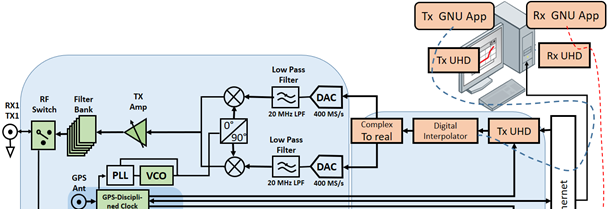
\includegraphics[scale=1]{Imagenes/Elementos-internos.png}
	\label{fig:Elementos-internos}
%	\captionsetup{justification=raggedright,font={scriptsize,bf,it}}
%	\caption*{fuente: https://www.ettus.com/content/files/USRP-E310-Product-Sheet.pdf \\
%		Nota: no es claro que el NI USRP 2920 tenga un banco de filtros como estos, pues no aparecen en los manuales}
\end{figure}

{\setlength{\parindent}{1pt}En la figura XXX se observa que en modo transmisión, el USRP usa un DAC con una frecuencia de muestreo de 400 MS/s. También se observa que cuenta con el bloque Digital Interpolator para adaptar la frecuencia de muestreo de la señal que le llega.  Pero al igual que ocurrió con el coeficiente de decimación, en el modo recepción, aquí el coeficiente de interpolación también en obligatoriamente un número entero de la forma:}

\begin{equation} \label{captres_dos}	
K_{i} = 2^{m}, donde m es entero positivo. 
\end{equation}


\subsection{El papel de GPS en un NI USRP.}

El papel del GPS consiste en usar una señal satelital, del sistema GPS para lograr que el VCO de cualquiera de los varios equipos genere una misma senoidal. Esto mejora enormemente la recepción de una señal transmitida con otro USRP similar, ya que no se presenta desfase entre la portadora usada en el transmisor y en el receptor. Pero esta opción solo la tienen los NI USRP-293x.\\

\subsection{Los filtros en un NI USRP.}

\subsection*{En la parte receptora} 
La siguiente figura presenta un ejemplo de la respuesta en frecuencia del banco de filtros, como no se tenía en el momento la información para el NI USRP 2920, se presenta la del NI USRP E-310, para que el lector tenga una idea de lo que ese banco de filtros significa.

\begin{figure}[h!]
	\captionsetup{justification = raggedright, singlelinecheck = false}
	\caption{Banco de Filtros de la parte receptora del NI USRP E-310.} 
	\centering
	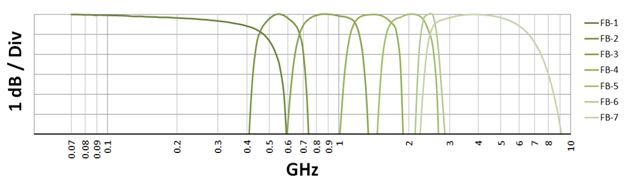
\includegraphics[scale=1]{Imagenes/Banco-filtros.png}
	\label{fig:Banco-filtros}
			\captionsetup{justification=raggedright,font={scriptsize,bf,it}}
			\caption*{fuente: https://www.ettus.com/content/files/USRP-E310-Product-Sheet.pdf \\
			Nota: no es claro que el NI USRP 2920 tenga un banco de filtros como estos, pues no aparecen en los manuales}
\end{figure}

El filtro a usar es seleccionado directamente por el Usuario P.\\

A manera de resumen, las especificaciones del receptor del NI USRP-2920 son  las siguientes: \\

\begin{itemize}
	\item [$\bullet$] La información más confiable sobre las especificaciones es la del	\textcolor{red}{\href{http://www.ni.com/pdf/manuals/376358a.pdf}{manual del equipo}}.
	\item [$\bullet$] Rango de frecuencias de 50 MHz a 2.2 GHz. (las bandas de radio FM, GPS, GSM, radar, ISM)
	\item [$\bullet$] Pasos de frecuencia $<$ 1 kHz
	\item [$\bullet$] Se usa un ADC de dos canales: 100 MS/s a 14 bits/muestra. Un canal es para la señal I y el otro para la señal Q, como se deduce de este \textcolor{red}{\href{http://www.ni.com/white-paper/13881/en/}{enlace}}
	\item [$\bullet$] El rango dinámico del ADC es 1 Vp-p. La potencia de entrada al ADC es no lineal pues varía con la frecuencia.
	\item [$\bullet$] Rata máxima real de muestreo I/Q: 25 MS/s a 16 bits/muestra; 40 MS/s a 8 bits/muestra. El manual aclara que este valor puede verse limitado aún más por las limitaciones del computador usado y por la velocidad de la conexión entre el USRP y el computador. A diferencia de la frecuencia de muestreo del ADC,este valor se refiere a la rata de muestreo a la que realmente puede funcionar el sistema en tiempo real. En otras palabras, si se intentara aprovechar los 100 MS/s que entrega el ADC, veríamos que el sistema se bloquearía o produciría errores, debido a que esa velocidad no es soportada por los bloques que siguen. 
	\item [$\bullet$] Ancho de banda máxima real: 20 MHz para 16 bits/muestra; 40 MHz para 8 bits/muestra.
	\item [$\bullet$] Nota 2: se deduce también que el Ancho de banda máxima instantánea en tiempo real, es el valor pasobandas que en términos reales se puede alcanzar, que representaremos como B. De modo que en bandabase, el ancho de banda es BW=B/2. Así toma sentido la frecuencia de muestreo que es Fs=2*BW=B. Por eso, vemos que en el caso de 8 bits/muestra, con 40 MS/s se alcanza un ancho de banda de 40 MHz. Eso es lo máximo que el equipo permite. Pero el Front-End al que tiene acceso el usuario P, es decir, el GRC, puede no tener la opción para programar este valor de 8 bits/muestra.
	\item [$\bullet$] El usuario P usualmente necesita un menor valor para la frecuencia de muestreo que entrega el USRP Source. Para satisfacer esa necesidad, el USRP Source cuenta con un diezmador. El problema es que el factor de diezmado no es cualquiera, sino que se aproxima al valor más cercano entre los siguientes: 8, 16, 32, 64, 128, 256, 512. 
\end{itemize}

Otras notas de interés para configurar el bloque de GNU radio conocido como USRP Source: \\

\begin{itemize}
	\item [$\bullet$] Para los usuarios P de Simulink es un poco confuso que el muestreo sea realizado por el ADC. Esto se entiende mejor si imaginamos que el ADC del usrp junto con el procesado que realiza luego el OSP, equivalen en Simulink a la interconexión de los bloques: filtro paso bajas, muestreador (con el bloque zero order hold), cuantizador (en caso de que la salida del USRP source sea configurada para  tipo entero). De modo que ADC+OSP lo que entregan es una señal, que usualmente veremos como una señal de valores decimales con un número finito de posibles valores. En otras palabras es la envolvente compleja de la señal que el usuario P desea capturar, pero en su versión muestreada y cuantizada, por lo tanto, esta señal pertenece al mundo físico.
	\item [$\bullet$] En Simulink de Matlab, el bloque USRP Source no pide frecuencia de muestreo sino coeficiente de decimación.
	\item [$\bullet$] El valor máximo de frecuencia de muestreo que se pudo programar sin problemas con un computador Core i7 fue de  fue de 20 MSps, que equivale a un ancho de banda pasobandas de 20 MHz. Pero con advertencias puede ser de 25 MSps. Teóricamente, con computadores mejor dotados se podría elevar más, pero sin pasar nunca de 50 MSps.
	\item [$\bullet$] Aunque la documentación dice que la frecuencia de muestreo cambia en función de número de bits por muestra que se elija, vimos que al menos el bloque USRP Source no brinda esta opción.
	\item [$\bullet$] Si el parámetro Ch0: Bandwidth se deja en cero, el ancho de banda del receptor usrp se sintoniza por defecto a una frecuencia cercana a la frecuencia de muestreo, porque se aplica el Teorema de Nyquist en versión bandabase.
	\item [$\bullet$] Otros parámetros del receptor del USRP de la serie N2920 son:
	\begin{itemize}
		\item [$\bullet$] La letra “N” se refiere a “Network”, debido a que usa puerto Gigabit  Ethernet para la unión PC-USRP
		\item [$\bullet$] La velocidad de los datos entre el PC y el USRP por el puerto Ethernet es de hasta 50 MS/s
		\item [$\bullet$] Se pueden unir varios USRP como si fuesen uno solo para escalar en capacidad
	\end{itemize}
\end{itemize}

\subsection{En la parte transmisora}
De manera similar, en la parte transmisora puede tenerse un banco de filtros como es el caso del NI USRP E-310, como se muestra en la Figura \ref{fig:Banco-e310}

\vspace{300px}
\begin{figure}[h!]
	\captionsetup{justification = raggedright, singlelinecheck = false}
	\caption{Banco de Filtros de la parte transmisora del NI USRP E-310.} 
	\centering
	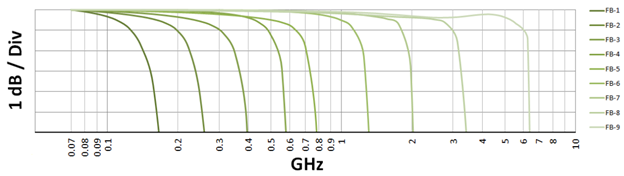
\includegraphics[scale=0.9]{Imagenes/Banco-e310.png}
	\label{fig:Banco-e310}
			\captionsetup{justification=raggedright,font={scriptsize,bf,it}}
			\caption*{fuente: https://www.ettus.com/content/files/USRP-E310-Product-Sheet.pdf}
\end{figure}

\subsection{Actividades de Caracterización del equipo}

Las especificaciones anteriores son datos tomados de la documentación del equipo NI USRP-2920. Sin embargo, una verificación práctica brinda resultados más reales, pues muchas veces los manuales tienen inconsistencias. Los siguientes son verificaciones realizadas:

\begin{itemize}
	\item [$\bullet$] Se programó el bloque USRP Source una tasa de muestreo de 20 MHz, para capturar una señal de ancho de banda pasobandas de 20MHz, que puede equivaler a todo el espectro de FM. También se le programó una salida de tipo Complex float32.  y esto se observó:
	\begin{itemize}
		\item [$\bullet$] Es algo perfectamente normal con un buen computador.
		\item [$\bullet$] Al correr el flujograma y observar los mensajes que aparecen en la ventana de texto inferior del GRC, dice lo siguiente: decimation=dsp-rate/samp-rate: 5=100 MHz/20MHz. Eso significa que la frecuencia de muestreo fija usada por el USRP es 100 MS/s
		\item [$\bullet$] Hay otro dato interesante en esa ventana de texto: The requested decimation is odd; the user should expect CIC rolloff. Select even decimation to ensure that a halfband filter is enable. Osea que se está pidiendo una decimación impar y que eso tiene consecuencias en que el usuario P no reciba exactamente lo que espera, hay un filtro que no queda bien cuadrado, entonces sugiere solicitar siempre decimación par para asegurar que se activa un filtro pasobajas con un ancho de banda que es la mitad del ancho de banda pasobandas programado en el bloque USRP Source.	
	\end{itemize}
	\item [$\bullet$] Se probó la misma configuración del USRP Source pero con salida tipo Complex Int16. Se observó que:
	\begin{itemize}
			\item [$\bullet$] Aparecen los mismos mensajes de texto, luego, la frecuencia de muestreo no se altera, es siempre 100 MS/s.
			\item [$\bullet$] Se probó la misma configuración con frecuencia de muestreo 10 MHz y salida Complex float32. Funcionó a las mil maravillas.
			\item [$\bullet$] Se probó la misma configuración con frecuencia de muestreo 25 MHz y salida Complex float32, con lo cual se produce una decimación igual a 4. Funcionó bien durante unos segundos, luego siguió funcionando, pero en la ventana de texto botando una advertencia de Error: error in pthread-setschedparam. Digo que siguió funcionando, pero porqué ví que en el osciloscopio la señal continuaba apareciendo. 
			\item [$\bullet$] Se probó la misma configuración con frecuencia de muestreo 100 MHz y salida Complex float32, con lo cual se produce una decimación igual a 1. No corre, la advertencia dice: The hardware does not support the requested RX sample rate: Target sample rate: 100MSps, Actual sample rate: 50 MSps. Osea que el tope de frecuencia de muestreo que podemos pedir es de 50 MHz, si pedimos más, el sistema redondea para entregar 50 MSps, si es que el computador los soporta. Pero hay que tener en cuenta que hasta la misma velocidad del puerto Gigabit Ethernet puede ser un problema.
			\item [$\bullet$] Se probó la misma configuración con frecuencia de muestreo 50 MHz y salida Complex float32, No corre, dice que: Unable to set the thread priority. Performance may be negatively affected. Error in pthread-setschedparam
			\item [$\bullet$] Se probó la misma configuración con frecuencia de muestreo 24 MHz y salida Complex float32. Funcionó con advertencias: Target sample rate: 24 MHz, Actual sample rate: 25 MHz. También mostró un error error in pthread-setschedparam
			
	\end{itemize}
\end{itemize}

%%%%%%%%%%%%%%%%%%%%%%%%%%%%%%%%%%%%%%%%%%%%%%%%%%%

\section{Cuidados con el uso de los equipos SDR}

Es importante leer las instrucciones sobre los cuidados que se deben tener con los equipos USRP. Usualmente estos mencionan los siguientes: \\

\begin{itemize}
	\item [$\bullet$] Previsión de cargas electrostáticas que pueden dañar su equipo.
	\item [$\bullet$] Póngase en conexión a tierra sosteniendo algo que esté aterrizado, como por ejemplo el chasis de su computador.
	\item [$\bullet$] Una conexión de transmisión/recepción en el mismo equipo debe realizarse con el cable suministrado y a través del atenuador de 30 dB suministrado. El atenuador debe conectarse directamente al puerto receptor.
	\item [$\bullet$] Se instala el software primero, antes de hardware.
	\item [$\bullet$] Si hace reinicio de PC, primero encienda el USRP, luego el PC.	
\end{itemize}

Los siguientes son los cuidados que demandan más atención por el peligro de poder dañar las tarjetas hijas:

\begin{itemize}
	\item [$\bullet$] El receptor es un dispositivo extremadamente sensible y puede dañarse o deteriorarse fácilmente por mal uso. Contrariamente, el transmisor es un equipo de alta potencia, si se compara con el receptor
	\item [$\bullet$] El uso natural del receptor sería el de recibir una señal inalámbrica que se ha propagado en la distancia y consecuentemente se ha atenuado sensiblemente. Una señal de este tipo no pone en peligro el receptor.
	\item [$\bullet$] Igualmente lo más natural sería usar el transmisor conectado a una antena para transmitir en la distancia.
	\item [$\bullet$] El problema es que en condiciones de laboratorio puede dársele otros usos al transmisor y al receptor, como estos:
	\begin{itemize}
		\item [$\bullet$] El transmisor se conecta directamente al receptor a través de un cable. En este caso, el riesgo es para el receptor pues puede llegar a recibir una potencia más alta que la que puede soportar. La prevención consiste en conectarle previamente al puerto del receptor la carga del atenuador de 30 dB.
		\item [$\bullet$] El transmisor se usa sin antena, por ejemplo para observar en un osciloscopio la señal que aparece en ese puerto. En este caso el receptor está en riesgo, pues la energía que necesita ser emitida por la antena puede devolverse al transmisor y quemar el MOSFET. Ese fenómeno se conoce como Onda Reflejada y consiste en que la energía que no pueda ser emitida por una antena se devuelve al transmisor.  Lo recomendable es que siempre se tenga una antena conectada al puerto del transmisor.
	\end{itemize}
\end{itemize}

%%%%%%%%%%%%%%%%%%%%%%%%%%%%%%%%%%%%%%%%%%%%%%%%%%%

\section{Razonamiento sobre el teorema de Nyquist en SDR}

El título de este capítulo no significa que el Teorema de Nyquist cambia con el uso de gnuradio. Solo está orientado a brindar las siguientes orientaciones claves para usar este concepto correctamente en gnuradio:

\begin{itemize}
	
	\item [$\bullet$] 	El Teorema de Nyquist dice que si un señal continua, banda base, tiene una ancho de banda BW, puede ser muestreada a una frecuencia de muestreo $F_{s}$ que que es mayor o igual a dos veces BW: $F_{s} \geq 2$ BW
	\item [$\bullet$] Una señal puede ser bandabase por naturaleza, por ejemplo la voz y la mayoría de los mensajes de información, pero también puede ser el resultado de hacer pasar una señal pasobandas, con un ancho de banda B, por un Down Converter. En este caso $BW = \frac{B}{2}$, por lo tanto el Teorema de Nyquist para este caso es así: $F_{s} \geq B	$
\end{itemize}

%%%%%%%%%%%%%%%%%%%%%%%%%%%%%%%%%%%%%%%%%%%%%%%%%%%%%%%


\section{Equipo SDR para soluciones en modo embebido}
\textcolor{red}{[Falta]}

%%%%%%%%%%%%%%%%%%%%%%%%%%%%%%%%%%%%%%%%%%%%%%%%%%%%%

\section{Un sistema de Radiodifusión AM}
[Aquí lo que se busca es llegar a usar el USRP, pero también poner todos los elementos que estaría en un sistema radiodifusión de verdad, como los filtros, etc. Si esos elementos ya se usaron en el capítulo de simulación, lo que resta es más que todo la configuración del USRP y métodos para realizar las pruebas, pruebas de propagación, etc. Tenemos la duda, si vale la pena pasar alguno de los subtemas al capitulo que habla de simulación en GNU Radio]

\subsection{Modelo de capas}
\subsection{La capa del mensaje}
\subsubsection{mensaje Monofónico}
\subsubsection{mensaje stereo}
\subsection{La capa de modulación}
\subsection{La capa de pre-canal}

%%%%%%%%%%%%%%%%%%%%%%%%%%%%%%%%%%%%%%%%%%%%%%%%%%

\section{Un sistema de Radiodifusion FM}
[Se tienen las mismas dudas identificadas en la radio difusion AM]
\subsection{Modelo de capas}
\subsection{La capa de modulación}
\subsection{La capa de pre-canal}
